\documentclass[main.tex]{subfiles}
\begin{document}
\subsection{Show that $[E_{\alpha},E_{\beta}]\propto E_{\alpha+\beta}$}\label{Qu6A}
To show this we make use of the Jacobi identity
\begin{align}
[H_i,[E_{\alpha},E_{\beta}]]&=-[E_{\alpha},[E_{\beta},H_i]]-[E_{\beta},[H_i,E_{\alpha}]]\\
&=[E_{\alpha},\beta_iE_{\beta}]+[\alpha_iE_{\alpha},E_{\beta}]\\
&=(\alpha_i+\beta_i)[E_{\alpha},E_{\beta}].
\end{align}
Also
\begin{equation}
[H_i,E_{\alpha+\beta}]=(\alpha_i+\beta_i)E_{\alpha+\beta}.
\end{equation}
This implies $[E_{\alpha},E_{\beta}]\propto E_{\alpha+\beta}$. Furthermore if $(\alpha_i+\beta_i)$ is not a root then $[E_{\alpha},E_{\beta}]=0$ and consequently $E_{\alpha+\beta}=0$.

\subsection{Calculate $[E_{\alpha},E_{-\alpha-\beta}]$}
We have $[E_{\alpha},E_{\beta}]=NE_{\alpha+\beta}$. Taking the h.c. we get $[E_{-\alpha},E_{-\beta}]=NE_{-\alpha-\beta}$. So,
\begin{align}
[E_{\alpha},E_{-\alpha-\beta}]&=\frac{1}{N}[E_{\alpha},[E_{-\alpha},E_{-\beta}]]\\
&=-\frac{1}{N}\left([E_{-\alpha},[E_{\alpha},E_{-\beta}]]+[E_{\beta},[E_{\alpha},E_{-\alpha}]]\right)\\
&=\frac{1}{N}[[E_{\alpha},E_{-\alpha}],E_{\beta}]\\
&=\frac{1}{N}[\alpha.H,E_{\beta}]\\
&=-\frac{1}{N}\alpha.\beta E_{-\beta},
\end{align}
where we have used the fact that $[E_{\alpha},E_{-\beta}]=0$ because $\alpha-\beta$ is not a root.

\subsection{Find the weights in the defining representation}
The simple lie algebra generated by $\sigma_a\otimes\mathbb{I}$, $\sigma_a\otimes\tau_1$, $\sigma_a\otimes\tau_3$, $\mathbb{I}\otimes\tau_2$. We take the Cartan subalgebra as $H_1=\sigma_3\otimes\mathbb{I}$, $H_2=\sigma_3\otimes\tau_3$.
\begin{equation}
H_1=\begin{pmatrix}1&0&0&0\\0&-1&0&0\\0&0&1&0\\0&0&0&-1\end{pmatrix},\quad H_2=\begin{pmatrix}1&0&0&0\\0&-1&0&0\\0&0&-1&0\\0&0&0&1\end{pmatrix}
\end{equation}
\subsubsection{Weights in the defining representation}
The eigenvalues of $H_1$ \& $H_2$ are $\lambda_1=\pm1$, $\lambda_2=\pm1$. Calculating the eigenvectors $H_kV_i=\lambda_{ik}V_i$.
Then the eigenvectors with their associated weights are
\begin{align}
\begin{pmatrix}1\\0\\0\\0\end{pmatrix}\rightarrow(1,1)\quad \begin{pmatrix}0\\0\\0\\1\end{pmatrix}\rightarrow(-1,1)\quad
\begin{pmatrix}0\\1\\0\\0\end{pmatrix}\rightarrow(1,-1)\quad \begin{pmatrix}0\\0\\1\\0\end{pmatrix}\rightarrow(-1,-1)
\end{align}

Plotting the weight diagram 
\begin{figure}[H]
\centering
\begin{tikzpicture}
\draw[->] (0,-3) -- (0,3) node[right] {$H_2$};
\draw[->] (-3,0) -- (3,0) node[right] {$H_1$};
\filldraw[black] (-1,-1) circle (2pt) node[left] {(-1,-1)};
\filldraw[black] (1,-1) circle (2pt) node[right] {(1,-1)};
\filldraw[black] (-1,1) circle (2pt) node[left] {(-1,1)};
\filldraw[black] (1,1) circle (2pt) node[right] {(1,1)};
\end{tikzpicture}
\end{figure}
 
\subsubsection{Weights of the adjoint representation}
The weights of the adjoint representation are given by the the roots of the algebra which we can deduce by looking at the difference in weights of the defining representation from part (a). The raising and lowering operators take us between the weights in part (a), they are: $E_{\pm2,0}$, $E_{\pm2,\mp2}$, $E_{\pm2,\pm2}$, $E_{0,\pm2}$.

Plotting the roots on the weight diagram
\begin{figure}[H]
\centering
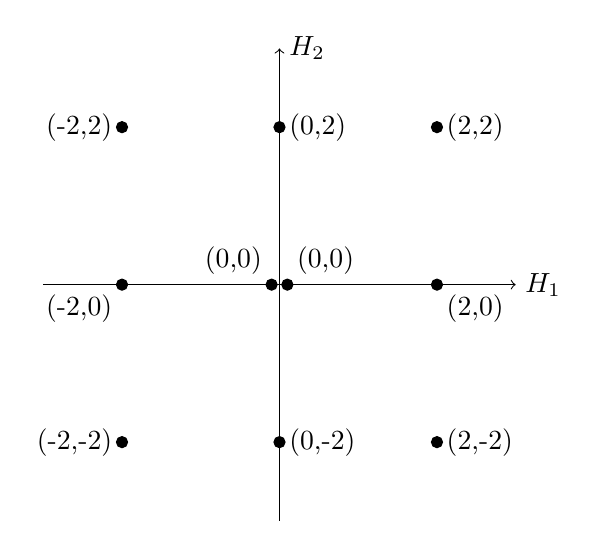
\begin{tikzpicture}
\draw[->] (0,-3) -- (0,3) node[right] {$H_2$};
\draw[->] (-3,0) -- (3,0) node[right] {$H_1$};
\filldraw[black] (0,2) circle (2pt) node[right] {(0,2)};
\filldraw[black] (2,2) circle (2pt) node[right] {(2,2)};
\filldraw[black] (2,0) circle (2pt) node[below right] {(2,0)};
\filldraw[black] (2,-2) circle (2pt) node[right] {(2,-2)};
\filldraw[black] (0,-2) circle (2pt) node[right] {(0,-2)};
\filldraw[black] (-2,-2) circle (2pt) node[left] {(-2,-2)};
\filldraw[black] (-2,0) circle (2pt) node[below left] {(-2,0)};
\filldraw[black] (-2,2) circle (2pt) node[left] {(-2,2)};
\filldraw[black] (-0.1,0) circle (2pt) node[above left] {(0,0)};
\filldraw[black] (0.1,0) circle (2pt) node[above right] {(0,0)};
\end{tikzpicture}
\end{figure}

\end{document}